\section{A Preprocessing Procedure For Identifying Jump Points}

The aim of the preprocessing 
is, for every node $n$ and every direction $\vec{d}$, 
to compute off-line the jump point 
and store it in a table $\jp$, 
such that, at runtime, the jump point $\jp[n][\vec{d}]$
may be retrieved automatically.  
The problem we face here 
is that the procedure that identifies the jump point 
needs to know the goal, 
which is unknown at preprocessing time.  
Therefore, we need 
to defensively insert additional jump point 
to ensure correctnes, 
but only add those that are really necessary 
to avoid clogging JPS.  

Given the node $n \in \mathcal{N}$ and the direction $\vec{d}$, 
the preprocessed jump point (PJP), 
$PJP(n,\vec{d}) \in \mathcal{N} \cup \{\varnothing\}$ 
is either a node $n' \in \mathcal{N}$ 
or a null value ($\varnothing$) which means that there is no PJP 
from node $n$ in direction $\vec{d}$.  

We now introduce the notion of a stop point, 
which intuitively corresponds to a node 
where the search should eventually stop, 
and next define the PJP as the first stop point.  

\begin{definition}\label{def::stop}
  The node $n'$ is a \emph{stop point} 
  from node~$n$ in direction~$\vec{d}$ 
  iff i) $n' = n + k \times \vec{d}$ for some positive integer $k$, 
  ii) for all $i \in \{0,\dots,k\}$, 
  $n + i \times \vec{d}$ is not an obstacle, 
  and iii) one of these conditions holds: 
  \begin{itemize}
  \item 
    $n'$ is forced, 
  \item 
    $\vec{d}$ is a diagonal move 
    and there exists a node $n_i = n' + k_i \times \vec{d_i}$ 
    which lies $k_i \in \mathbf{N}$ steps 
    in direction $\vec{d_i} \in \{\vec{d_1},\vec{d_2}\}$ 
    such that $n'$ is forced, 
    or
  \item
    $n' + \vec{d}$ is an obstacle.  
  \end{itemize}
\end{definition}

Compared to the original jump point definition, 
there are two differences: 
\begin{itemize}
\item 
  the goal is not a stop point (because it is unknown at this stage), 
\item 
  the move just before hitting an obstacle is a jump point: 
  the reason for that is that we want 
  to force the search algorithm to explore every ``hideaway'' in the map.  
\end{itemize}

The PJP is then defined as the first stop point: 
\begin{definition}
  From node~$n$ and direction~$\vec{d}$, 
  the \emph{preprocessed jump point} is the stop point $n'$ 
  from node~$n$ in direction~$\vec{d}$ 
  that minimises the value $k$ such that $n' = n + k \times \vec{d}$ 
  if such a stop point exists, or $\varnothing$ otherwise.  
\end{definition}

\paragraph*{}

The preprocessed table cannot be used exclusively 
to determine the jump point.  
Because the table was generated 
at a time where the goal was unknown, 
some additional reasonning is necessary to determine the jump points.  

The jump points are essentially locations 
where the search algorithm should consider 
stopping moving in the current direction.  
The reasons for stop are 
i) that the goal has been reached, 
ii) that the goal is now accessible in a different direction, 
iii) that an obstacle has been circumvented 
offering access to a new part of the grid.  
Those reasons are not mutually exclusive.  
The last reason is delt with 
by the table as it has been built.  
However, the first two reasons need to be considered.  

Consider a node~$n$ and a direction~$\vec{d}$ 
such that the PJP~$\jp[n][\vec{d}]$ passes through goal~$g$.  
The jump point should be at $g$.  

Consider now a node~N, a diagonal direction~$\vec{d}$, 
and the PJP~Y$ = \jp[$N$][\vec{d}]$ 
such that the segment N--Y cuts a vertical or a horizontal line 
that is drawn from goal~G and that stops at obstacles 
(see Figure~\ref{fig::inserted}).  
Then the jump point should be at the first location~J
where the line cuts the segment.  
(Observe that the first condition described above 
is a special case of the second condition.)

\begin{figure}[ht]
  \begin{center}
  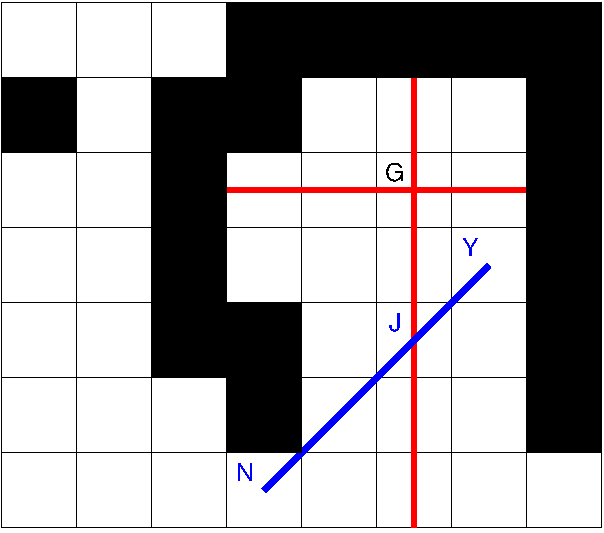
\includegraphics[scale=0.7]{inserted}
  \end{center}
  \caption{Because the segment between the node N 
    and its expected successor Y 
    is cut by the red line, 
    the jump stops at J.}
  \label{fig::inserted}
\end{figure}

We now formalise these statements.  

\begin{definition}\label{def::insertion}
  Let $n$ be a node, 
  let $\vec{d}$ be a direction, 
  let $y = \jp[n][\vec{d}]$ be the PJP from $n$ in direction~$\vec{d}$, 
  and let $g$ be the goal, 
  the \emph{on-line jump point} from $n$ in direction~$\vec{d}$ 
  is defined as follows: 
  \begin{itemize}
  \item 
    if $y = \varnothing$, then $\varnothing$
  \item 
    if there exists a node $j$ between $n$ and $y$ 
    and there exists $k \in \mathbf{N}$ 
    and $\vec{d_i} \in \{\vec{d_1},\vec{d_2}\}$ 
    such that $g = j + k \vec{d_i}$ 
    and for all $k' \in \{1,\dots,k\}$, $j + k' \vec{d_i}$ 
    is not an obstacle, 
    then $j$, 
  \item 
    else $y$.  
  \end{itemize}
\end{definition}

\begin{lemma}
  If the jump point from node~$n$ in direction~$\vec{d}$ is $j$, 
  then the on-line jump point from $n$ in $\vec{d}$ is $j$.  
\end{lemma}

\begin{proof}
  We consider all three instances that define $j$.  
  Notice that, for all three cases, 
  there is no node $n'$ between $n$ and $j$ 
  such that $n'$ is the goal or $n'$ satisfies 
  one of the first two conditions in Definition~\ref{def::stop} 
  (otherwise, $j$ would be this $n'$).  
  \begin{itemize}
  \item 
    Assume $j$ is the goal.  
    Then the node $y = \jp[n][\vec{d}]$ 
    is such that $j$ is in the segment $n$--$y$ 
    (because in the worst case, 
    $y$ is the last node before an obstacle is hit).  
    Therefore according to Definition~\ref{def::insertion}, 
    the on-line jump point is $j$.  
  \item 
    If $j$ has a forced moved, then 
  \item 
    If $j$ is a node...
  \end{itemize}
\end{proof}

Because this approach is equivalent to JPS, 
the following corollary holds.  

\begin{corollary}
  Searching with jump point pruning 
  as presented in Definition~\ref{def::insertion} 
  always returns an optimal solution.  
\end{corollary}

%%% The search algorithm uses the PJP table
%%% to accelerate the search.  
%%% Because the table was generated 
%%% at a time where the goal was unknown, 
%%% the algorithm must still check for the goal.  
%%% 
%%% \begin{algorithm}
%%%   {\bf Require:}
%%%     $x$: current node,
%%%     $\vec{d}$: direction,
%%%     $g$: goal,
%%%     $\jp$: the PJP table
%%%   \begin{algorithmic}[1]
%%%   \STATE $n \leftarrow \jp[x][\vec{d}]$
%%%   \IF{$n = \varnothing$}
%%%     \STATE {\bf return} $\varnothing$
%%%   \ENDIF
%%%   \IF{$g$ is between $x$ and $n$}
%%%     \STATE {\bf return} $g$
%%%   \ENDIF
%%%   \STATE {\bf return} $n$
%%%   \end{algorithmic}
%%%   \caption{Function \emph{jump\_straight}}
%%% \end{algorithm}
%%% 
%%% \begin{algorithm}
%%%   {\bf Require:}
%%%     $x$: current node,
%%%     $\vec{d}$: direction,
%%%     $g$: goal,
%%%     $\jp$: the PJP table
%%%   \begin{algorithmic}[1]
%%%   \STATE $n \leftarrow \jp[x][\vec{d}]$
%%%   \IF{$n = \varnothing$}
%%%     \STATE {\bf return} $\varnothing$
%%%   \ENDIF
%%%   \IF{the row of $g$ cuts the segment $x$--$n$}
%%%     \STATE Let $y$ be the node where the segment is cut
%%%     \STATE Let $\vec{d_i}$ be the horizontal direction 
%%%       in $\{\vec{d}_1,\vec{d}_2\}$
%%%     \STATE $z \leftarrow \jp[y][\vec{d_i}]$
%%%     \IF{$z \neq \varnothing\ \land\ g$ is between $y$ and $z$}
%%%       \STATE {\bf return} y
%%%     \ENDIF
%%%   \ENDIF
%%%   \IF{the column of $g$ cuts the segment $x$--$n$}
%%%     \STATE Let $y$ be the node where the segment is cut
%%%     \STATE Let $\vec{d_i}$ be the vertical direction 
%%%       in $\{\vec{d}_1,\vec{d}_2\}$
%%%     \STATE $z \leftarrow \jp[y][\vec{d_i}]$
%%%     \IF{$z \neq \varnothing\ \land\ g$ is between $y$ and $z$}
%%%       \STATE {\bf return} y
%%%     \ENDIF
%%%   \ENDIF
%%%   \STATE {\bf return} $n$
%%%   \end{algorithmic}
%%%   \caption{Function \emph{jump\_diag}}
%%% \end{algorithm}

% EOF
